\documentclass[12pt, notitlepage]{article}
\usepackage[margin=4cm]{geometry}
\usepackage{hyperref}
\usepackage[english]{babel}
\usepackage{tocloft}
\usepackage{setspace}
\usepackage{graphicx}
\usepackage{caption}
\usepackage{subcaption}
\usepackage{listings}
\usepackage{float}
\usepackage{tabularx}
\usepackage[ruled,vlined]{algorithm2e}
\usepackage[numbers]{natbib}
\usepackage[style=american]{csquotes}
\usepackage{paralist}

\setcounter{tocdepth}{4}
\cftsetindents{paragraph}{1cm}{0cm}


\title{TitlePage}
\author{Stefan Gamerith\\\\
		\emph{Student ID: 0925081}}

\begin{document}
	\maketitle
	\thispagestyle{empty}
	\newpage
\setcounter{page}{1}

\section{Problem Definition}
The advance of embedding Information Technology into all kinds of electronic devices and connecting them to collect and exchange data imposes new challenges of handling the increasing amount of data. Although many problems can be solely solved by machines only, there are certain tasks where humans perform better than computers. In \emph{Crowdsourcing} collective human intelligence~(the crowd) is used to solve complex tasks. \citet{yuen2011survey}~grouped crowdsourcing applications into 
\begin{inparaenum}[1)]
		\item Voting Systems,
		\item Information Sharing Systems,
		\item Games with a purpose~(GWAP) and
		\item Creative Systems
\end{inparaenum}. 
First, Voting Systems like Amazon Mechanical Turk~(MTurk)~\footnote{https://www.mturk.com/} use majority voting to consider the answer with the highest number of votes as the correct one. Second, Information Sharing Systems enable users to share and distribute knowledge among the crowd. Third, Games with a purpose~(GWAP) is another application of crowdsourcing where crowd~workers contribute by playing a small game in order to solve some meaningful tasks. Fourth, Creative Systems include tasks like labeling an image, writing algorithms or editing text. 

An inherent factor of the Semantic Web is its large amount of Linked Data~(e.g. DBpedia~\cite{lehmann2015dbpedia}). Semantic technologies have emerged in various application including domain modeling, data integration, enhanced search and content management~\cite{semantic-web-usecases}. Managing Semantic Web tasks is considered resource intensive and often requires human involvement due to its knowledge intensive and context specific nature. On the other side Crowdsourcing aims at solving simple and small tasks~(microtasks) in a cost-effective way. However, \citet{sarasua2015crowdsourcing} shows major research challenges and opportunities in combining Crowdsourcing and Semantic Web technologies. The most important challenges include 
\begin{inparaenum}[1)]
		\item task and workflow design,
		\item managing the quality of contributions,
		\item handling multiple Crowdsourcing genres and 
		\item finding and managing the right crowd
\end{inparaenum}.
Whereas research shows that breaking task into smaller pieces and formulating the right questions to ask the crowd has a huge impact on the outcome of overall Crowdsourcing task, it is equally important to establish a model which formally defines the required quality and skills to perform tasks. Also, there exists no general guidelines when and under which settings small crowds with domain experts, large crowds with less qualified crowd workers or a mixed approach performs better. However, \citet{mortensen2013developing} concluded that average crowds perform on par with domain experts in "common sense" application domains, if crowd workers are carefully selected by qualification tests and tasks are presented in the simplest possible form. Although their experiments revealed that solving domain specific tasks (e.g. classification of diseases) requires good context and background knowledge, it was not further investigated how contextual information can be added in an automated manner. 

This work investigates this limitation by examining what kind context is needed to get better results, what would be the improvements in the overall workflow and how does the architecture of a concrete implementation look like. To answer the second question, a detailed evaluation study on selected domains and ontologies is conducted.

As a practical part, an extension of the existing \emph{uComp~Protege~Plugin~\cite{wohlgenannt2016crowd}} will be implemented. This plugin uses "embedded crowdsourcing" to verify properties of generic ontologies. In particular, it supports verification of Relation Correctness~(T2), Relation Type~(T3) and Domain Relevance~(T4). It achieves good results but their quality could be improved if concepts sent for crowdsourcing were better documented with relevant context. 

\section{Expected Result}
% -) Give a bit of explanation why each RQ is useful
% -) Move relevant results under each RQ
% -) Group Research questions with results
% -) Rephrase Research Questions (RQ1 - RQ3) to results (R1 - R3)

Based on the problem definition above, the following research questions are addressed in this thesis:
\paragraph{RQ1}~\textbf{What are the requirements for an extension of the uComp Protege plugin for adding contextual information to crowdsourcing tasks?}\\
\paragraph{RQ2}~\textbf{What approaches are applicable to facilitate the provision of contextual information for crowdsourcing tasks?}\\
\paragraph{RQ3}~\textbf{Does the proposed extension outperform the existing one on a selected set of ontologies?}\\
This thesis make use of empirical and exploratory approaches strengthening the confidence in answering the research questions. The following results are planned:
\begin{itemize}
	\item Functional and non-functional requirements for building an extension of the uComp Protege plugin.
	\item A detailed study of various options for enhancing crowdsourcing tasks with contextual information.
	\item A designed, implemented and evaluated extension of the uComp Protege plugin.
	\item An in-depth evaluation on the performance of the proposed extension.
	\item A reduction in costs and working time in crowdsourcing tasks while improving quality results from crowds.
\end{itemize}
\section{Methodological Approach}
% 	-) Remove sections, use paragraphs instead (or description lists)
% 	-) Make reference to each RQs
% 	-) Extend evaluation part 
%		*) Add references to ontologies that we already use
%		*) Bootstrapped based evaluation will be performed to make sure that the obtained results are generalizable 
% 	-) Add a picture about the concrete solution (at the end of the section) as we discussed 


The expected results are derived from the following methodology and approach:
\subsection{Literature Research}
For a complete picture on different approaches of how contextual information can be used to improve crowdsourcing tasks, an extensive literature research will be performed. For example one approach from a different research area but also applicable with focus on solving crowdsourcing tasks is ontology matching based on neighboring nodes~\cite{hoffmann2010context}. Although \emph{RQ2} will be addressed directly by this task, literature study is done continuously throughout the whole thesis. 
\subsection{Identify requirements}
Requirements for building an extension of the uComp Protege plugin will be collected by evaluating and extending the requirements of the existing approach~\cite{wohlgenannt2016crowd}. Grouped and evaluated requirements form a basis for choosing the most promising approach for the implementation.
\subsection{Identify different approaches for the implementation}
Based on the insights from literature research, various options for building the extension will be proposed. Each approach will be described in detail, concluding with estimated integration efforts. Based on this estimation, the actual development of the extension will be performed. 
\subsection{Integrate approach in the uComp Protege plugin}
The practical part of this thesis includes extending the uComp Protege plugin to take contextual information into account for performing crowdsourcing tasks. This extension implements all gathered requirements from former requirement analysis. In addition, we will give an overview of the overall plugin architecture as well as the crowdsourcing workflow. 
\subsection{Evaluate performance metrics}
To justify the improvements in a typical ontology engineering setting, a detailed evaluation based on the metrics in~\cite{wohlgenannt2016crowd} will be conducted. More specifically, evaluation metrics include the working time for an ontology engineer, task costs, task duration, data quality and scalability.  

\section{State of the art}
% Needs extension:
% 	-) 1 paragraph about crowdsourcing
% 	-) 1-3 paragraph about crowdsourcing in Semantic Web and concrete life-cycle stages in ontology engineering (based on SWJ table)
%	-) Describe uComp plugin and need for context [ok]
%	-) Add related work about context [Mortensen]
%	-) Describe related work for proposed approaches [ok].
%	-) (Probably move possible solutions to methodology)

The initial architecture for improving ontology engineering tasks with the help of crowdsourcing that will be used as a baseline for this thesis was introduced by \citet{wohlgenannt2016crowd}. The authors reported that \enquote{its use reduces the working times for the ontology engineers 11 times, lowers the overall task costs by 40\% to 83\% depending on the crowdsourcing settings used and leads to data quality comparable with that of tasks performed by ontology engineers.} The overall workflow ranging from task specification to result interpretation and presentation used by the tool is shown in Figure~\ref{fig:ucomp_workflow}.
\begin{figure}[H]
	 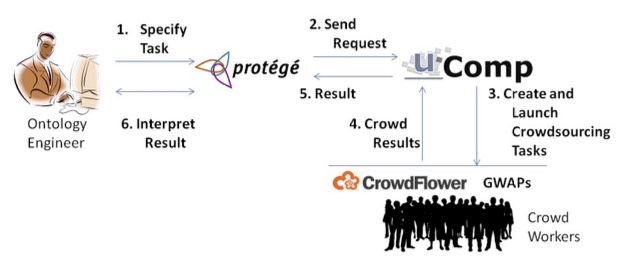
\includegraphics[width=\textwidth]{graphics/ucomp_workflow}
	 \caption{Overall workflow of the uComp Protege Plugin~\cite{wohlgenannt2016crowd}}\label{fig:ucomp_workflow}
\end{figure}

We limit our research to two related approaches described in the next paragraphs. Even though these were applied in different research contexts, applicability can be extended to adding contextual information to crowdsourcing tasks.

An area of interest is ontology matching. \citet{hoffmann2010context} states that \enquote{the context of an ontology can be given by its relations with other ontologies}. Hence, ontology matching is the task of putting ontologies in context whereas content based matching uses its metadata~(e.g. comments, labels, properties, \ldots) to compare ontologies. The context-based matcher Scarlet, first introduced by~\citet{sabou2008scarlet} and extended by~\citet{hoffmann2010context} combines various parameters of context-based matching such as the kind of ontologies that will be used, the method to choose ontologies to anchor concepts, the method to contextualize, the method to aggregate distinct results. 

Another area of interest is Question~Answering~Systems~(QA-Systems). Instead of using a formal query language like SPARQL~\cite{harris2013sparql}, QA-Systems process queries written in natural language. A rather complete overview of QA-Systems in the context of the Semantic Web covering major challenges is given by~\citet{hoffner2016survey}. They identified several challenges such as \emph{Lexical Gap}, \emph{Ambiguity}, \emph{Multilingualism}, \emph{Complex Queries}, \emph{Distributed Knowledge} and \emph{Procedural-,~Temporal-~and~Spatial~Questions}. They concluded that these challenges were subject of active research, leaving room for future improvements. 

\section{Relation to Software Engineering \& Internet Computing}
Researching, evaluating, developing, analyzing and verifying are important skills in the study \emph{Software Engineering \& Internet Computing}, matching the required skillset for answering the research questions in this thesis. Moreover, the development of an extension of the uComp Protege plugin requires an in-depth understanding of all phases of the Software Development Lifecycle, including Requirement~Analysis, Design, Implementation and Maintenance. Furthermore, an overall understanding of scientific principles and approaches as well as advanced knowledge of ontologies and related concepts is necessary. Therefore the qualification profile in the study of \emph{Software Engineering \& Internet Computing} is well covered. 

The following courses in the study of \emph{Software Engineering \& Internet Computing} are relevant:
\begin{itemize}
	\item 183.243 Advanced Software Engineering (PR)
	\item 180.456 Advanced Software Engineering (VO)
	\item 188.399 Introduction to Semantic Web
	\item 188.409 Requirements Engineering and Specification
\end{itemize}

\newpage
\bibliography{literature}
\bibliographystyle{plainnat}

\end{document}